% =====================================================================
%  Aggregate Task Success Hides the Signal  --  IEEE conference
%  format (IEEEtran), 4 pages. Paper C1.
%  Source of truth: paper/paper-1-dispersion-ceiling.md
%  Plan:           paper/PLAN-3-paper-split.md
%  Build: pdflatex paper-1-dispersion-ceiling-ieee.tex   (x2)
%
%  Reference metadata: every DOI below was resolved against the
%  Crossref REST API on 2026-10-10; [6] and [7] remain PARTIAL and
%  are flagged inline. See paper/reference-audit.md.
% =====================================================================
\documentclass[conference]{IEEEtran}

\usepackage[T1]{fontenc}
\usepackage[utf8]{inputenc}
\usepackage{times}
\usepackage{amsmath}
\usepackage{amssymb}
\usepackage{booktabs}
\usepackage{array}
\usepackage{graphicx}
\usepackage[hidelinks]{hyperref}

\newcommand{\todo}{\mbox{\textit{[\ldots]}}}

% tighter float/caption spacing to reach the 4-page target
\setlength{\textfloatsep}{6pt plus 2pt minus 2pt}
\setlength{\floatsep}{4pt plus 2pt minus 2pt}
\setlength{\intextsep}{5pt plus 2pt minus 2pt}
\setlength{\abovecaptionskip}{3pt}
\setlength{\belowcaptionskip}{0pt}

\begin{document}

\title{Aggregate Task Success Hides the Signal:\\ Per-Task Dispersion and Ceiling Effects\\
in Formative Usability Evaluation}

\author{
\IEEEauthorblockN{Meutia Braniwati$^{1}$, Bagaskoro Saputro$^{2}$, Aditya Paramananda$^{3}$, Freysia Chandra Saliman$^{4}$, Stephanie Evangelina Pramudito$^{5}$, and Tan, Michael Wilson Setiawan$^{6}$}
\IEEEauthorblockA{$^{1}$BINUS School of Design --- Visual Communication Design, Jakarta, Indonesia}
\IEEEauthorblockA{$^{2}$BINUS School of Computer Science --- Computer Science}
\IEEEauthorblockA{$^{3}$BINUS School of Information Systems --- Information Systems, Jakarta, Indonesia}
\IEEEauthorblockA{$^{4}$BINUS School of Computer Science --- Computer Science, Semarang, Indonesia}
\IEEEauthorblockA{$^{5}$BINUS School of Design --- Visual Communication Design, Semarang, Indonesia}
\IEEEauthorblockA{$^{6}$BINUS School of Information Systems --- Information Systems, Semarang, Indonesia}
\IEEEauthorblockA{Corresponding author: Meutia Braniwati, meutia.braniwati@binus.ac.id}
}

\maketitle

\begin{abstract}
Formative usability studies almost always report an aggregate task-success
rate. We argue that this summary is structurally lossy and demonstrate the
loss on complete real data rather than by simulation. Ten participants
completed eight standardised tasks across two moderated rounds, yielding
eighty task attempts, Single Ease Question (SEQ) scores on a 7-point scale,
and observer commentary, for a high-fidelity Indonesian-language home-services
marketplace prototype. Aggregate results are strong: \textbf{93.75\% task
success (75/80)} and \textbf{mean ease $M=6.56$, $SD=1.05$}. We argue both
numbers are close to uninformative. Computing dispersion per task shows
\textbf{four of the eight tasks saturated at $SD\leq0.42$}---they can no
longer distinguish a good design from a very good one. Only one task,
locating the FAQ and contact channel, produced meaningful spread
($M=5.70$, $SD=2.11$, full 1--7 range), and it is also the lowest-scoring.
A matched pair of discovery tasks isolates a further effect: a well-labelled
category was found without difficulty ($M=6.80$, $SD=0.42$) while a
near-synonymous label drew a 0.60 drop with triple the variance
($M=6.20$, $SD=0.92$), separating a taxonomy defect from a layout defect. We
further report that the two instrumented \textbf{defect probes were the only
tasks immune to saturation}, which suggests a practical rule: every formative
task set needs at least one probe that is expected to fail. We recommend
reporting per-task dispersion and probe results rather than totals, and we
publish the five provenance defects that constrain the conclusion.
\end{abstract}

\begin{IEEEkeywords}
usability testing, Single Ease Question, ceiling effect, dispersion, formative
evaluation, task success, measurement granularity, think-aloud
\end{IEEEkeywords}

\section{Introduction}

Household maintenance services in Indonesia---air-conditioner cleaning,
plumbing leak repair, pump servicing, septic tank suction---are dominated by
micro and small enterprises whose customer acquisition still runs through
spanduk (street banners), printed leaflets, and vehicle stickers \cite{tianti}.
The channel has structural properties that are easy to overlook because they
are invisible to the firm as well as the customer: a fixed physical area,
which caps how much information can be presented; no record of prior work; and
no price, which is negotiated privately and therefore unverifiable in advance.

A web interface removes the area constraint. It does not follow that the
resulting interface is good, and it certainly does not follow that it is
measurable. Most formative evaluations report a headline success rate, and a
headline success rate is a lossy summary of a multidimensional, per-task,
per-participant result.

This paper's contribution is to show, on complete real data, \textbf{how much
a headline success rate can hide.} We find a 93.75\% success rate coexisting
with four saturated tasks that can no longer generate evidence, one task whose
ratings span the entire scale, and a service taxonomy that misleads
participants who are otherwise fluent. Our practical recommendation follows
directly: \textbf{formative evaluation should report per-task dispersion and
defect-probe results, not just totals.}

\subsection{Research questions}

\begin{itemize}
\item \textbf{RQ1.} With what ease do young adult users complete a standardised
service-discovery and booking task sequence?
\item \textbf{RQ2.} Which tasks discriminate between participants, and which
are saturated?
\item \textbf{RQ3.} How can a task instrument be constructed so that some
tasks remain informative even when the design is strong?
\end{itemize}

\subsection{Related work}

Task-based design and evaluation of e-commerce interfaces is well established
in the Indonesian literature \cite{dinata}, and Tianti et al.~\cite{tianti}
demonstrate a small-business website raising promotional reach for a catering
MSME. Sunarso et al.~\cite{sunarso} provide evidence that visual content
raises attraction and conversion in MSME digital marketing. We adopt the
underlying premise while declining to import effect sizes measured on
different stimuli.

The Single Ease Question (SEQ) is a widely adopted post-task instrument: one
7-point item administered immediately after each task attempt, whose only
requirement is that the task be defined in terms the participant can recognise
\cite{sauro}. We adopt it for breadth---one comparable number per
attempt---while noting a trade-off our own data exposes sharply
(Sec.~III-B): SEQ is a \emph{mean} measure, and means conceal precisely the
information a formative study needs. Reporting the mean alone would have led
us to describe this prototype as uniformly easy, which Sec.~III-E shows it is
not.

Our argument is a special case of a general problem in measurement: a summary
statistic computed over heterogeneous items can be dominated by items carrying
little information while masking the items that carry all of it. Ceiling
effects are the standard psychometric term for this, and they are widely
discussed in survey research and adaptive testing, where item saturation is a
known threat to item-response estimation. What appears to be missing from HCI
practice is the routine reporting of dispersion at the \emph{task} level, as
opposed to the study level. A matched pair of tasks differing in exactly one
property is a standard identification strategy \cite{experimental}; we use one
below to separate a taxonomy defect from a layout defect.

Heuristic inspection \cite{nielsen} and its Indonesian applications
\cite{perdanakusuma,febriyanthi} are complementary but operate on a different
object: the code, not the experience. The convergence between the two methods
is examined in our companion papers.

\subsection{Scope and contributions}

This is a \emph{formative} evaluation of a single prototype build. No variable
measuring conversion, revenue, bounce rate, cognitive load, or trust change was
instrumented, and we make no claim about any of them. Our contributions are: a
per-task dispersion analysis of a complete evaluation; a matched-pair design
that converts a vague complaint into a specific diagnosis; a demonstration
that defect probes are the saturation-immune component of a task instrument;
and a candid account of five provenance defects.

\section{Methods}

\subsection{Prototype under test}

A high-fidelity React prototype, localised into Indonesian, implementing
service discovery with search and category filtering, service detail pages, a
four-stage checkout (summary $\rightarrow$ schedule $\rightarrow$ address
$\rightarrow$ payment), a confirmation/invoice view, technician tracking, and
an FAQ/contact area. Two properties were left unchanged during the study
because they bear directly on our research questions: prices render in
\textbf{USD} while the interface is Indonesian-language, and service
descriptions include \textbf{technician-internal procedure content} intended
for engineers rather than customers.

\subsection{Participants and disclosure}

Ten participants were recruited and tested in two rounds of five, identified
only by anonymous codes (P01--P05, P06--P10). Sessions were conducted in
Semarang, Central Java, between 1 and 30 October 2026.

\emph{Disclosure on demographics.} Participants were Gen Z, aged \textbf{19--21}, verified
against their national ID cards by the research team at recruitment and confirmed for all
ten. No date of birth was transcribed into the research data, as a privacy measure; the age
range is recorded here as an aggregate. Gender and occupation were not collected. The sample
is therefore described as \emph{Gen Z users recruited purposively} and we make
\textbf{no representativeness claim} beyond that description.

\subsection{Tasks}

Eight tasks spanning the booking flow (Fig.~\ref{fig:tasks}). T1 and T2 are a
\emph{matched} discovery pair differing only in service category.
\textbf{T6 and T7 are defect probes}---tasks with explicit failure criteria,
designed so that a correct prototype yields failures rather than successes.

\begin{figure}[t]
\centering
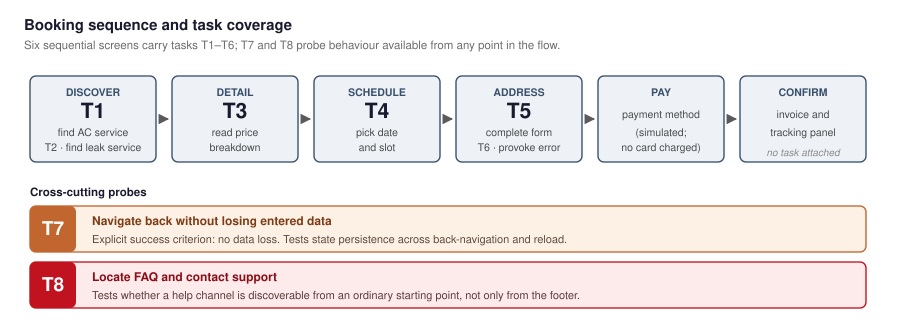
\includegraphics[width=\columnwidth]{figures/p1-fig1-task-sequence}
\caption{The eight-task instrument mapped onto the prototype's booking
sequence. Six sequential screens carry T1--T6; T7 and T8 probe behaviour
available from any point in the flow.}
\label{fig:tasks}
\end{figure}

\begin{table}[t]
\caption{Task instrument. T6 and T7 are defect probes.}
\label{tab:tasks}
\centering
\begin{tabular}{@{}cl@{}}
\toprule
Code & Task \\
\midrule
T1 & Locate the air-conditioner cleaning service \\
T2 & Locate the leak-detection service (matched to T1) \\
T3 & Read the detailed price breakdown \\
T4 & Select a booking date and time slot \\
T5 & Complete the address form \\
T6 & Trigger and identify a validation error (\textbf{probe}) \\
T7 & Navigate back without losing data (\textbf{probe}) \\
T8 & Locate FAQ / contact support \\
\bottomrule
\end{tabular}
\end{table}

\subsection{Measures and procedure}

\emph{Task outcome:} completed / completed with assistance / not completed,
against a written criterion per task. \emph{SEQ:} 1 = \emph{very difficult}
\ldots\ 7 = \emph{very easy}, immediately after each attempt. \emph{Observer
commentary:} notes on confusion, verbalised expectations, and unsolicited
suggestions.

Sessions were moderated with concurrent think-aloud. Screen and audio recording was conducted with the
consent of all ten participants and is stored under institutional control, scheduled for deletion on
1 January 2027; \textbf{the recordings were not used in this analysis}, and all qualitative material
available to it is therefore observer paraphrase, not verbatim transcript. We use quotation marks in
this paper only for source documents, never for participant speech.

\subsection{The completion-rate dispute, and how we resolved it}

Completion was coded during sessions and recorded as 39/40 (round 1) and
40/40 (round 2). Both source recap sheets then appended an auditor note that
specific attempts should have been coded failures: round~1, two T6 attempts
recorded as successes although the criterion was \emph{find the validation
message} and the notes state the participants did not find it; round~2, one T6
attempt recorded as a success although the note reads ``user did not find any
error,'' and another reaching confirmation with a street address consisting
only of the characters \texttt{(}\ and \texttt{)}.

This is a genuine interpretive disagreement about whether failure on a
\emph{sub-criterion} constitutes task failure, not an arithmetic error. Rather
than adopt either position silently, \textbf{we report the auditor-corrected
figures as the headline and present the as-recorded figures as a sensitivity
analysis} (Sec.~III-A).

\section{Results}

\subsection{Aggregate task success}

\begin{table}[t]
\caption{Task success, both codings.}
\label{tab:success}
\centering
\begin{tabular}{@{}lccc@{}}
\toprule
 & Round 1 & Round 2 & Combined \\
\midrule
As recorded      & 39/40 (97.5\%) & 40/40 (100 \%) & 79/80 (98.75 \%) \\
Corrected (head) & 37/40 (92.5 \%) & 38/40 (95.0 \%) & 75/80 (\textbf{93.75 \%}) \\
\bottomrule
\end{tabular}
\end{table}

Table~\ref{tab:success}. All five failures occurred at T6 or T8. A rate above
90\% would ordinarily indicate a largely successful design. \textbf{We do not
read it that way}, for two reasons. First, the T6 success criterion was
permissive---a permissive criterion inflates the aggregate, so the headline
number is an upper bound on its own reliability. Second, and decisively,
success is \emph{ceiling-bound}: four tasks were near-universally completed, so
the metric cannot discriminate between design states.

\subsection{Ease, and why the mean is not the finding}

Overall SEQ: \textbf{$M=6.56$, $SD=1.05$} ($n=80$ task-level ratings), median
7. Distribution: 62 ratings of 7, 10 of 6, 4 of 5, 1 of 4, 2 of 3, 1 of 1.
Per-task means and dispersions are given in Fig.~\ref{fig:seq} and
Appendix~\ref{app:matrix}.

\begin{figure}[t]
\centering
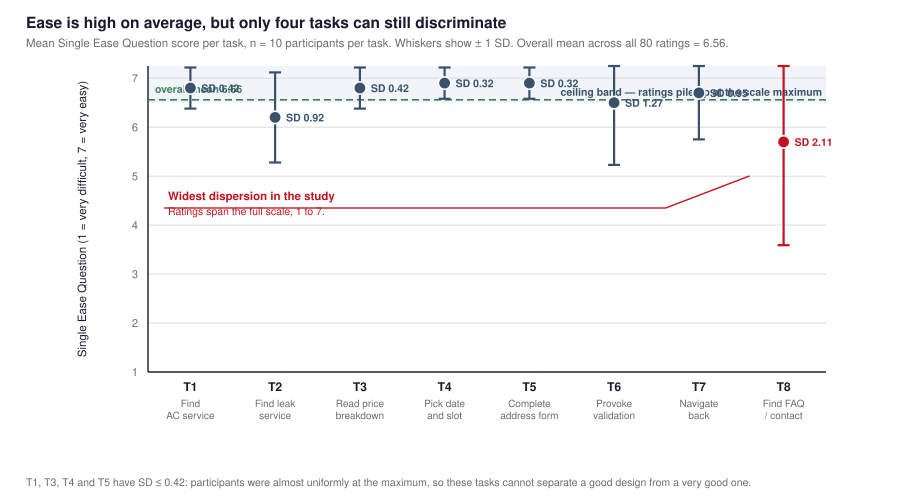
\includegraphics[width=\columnwidth]{figures/p1-fig2-seq-ceiling}
\caption{Mean SEQ per task with $\pm1$ SD whiskers. Four tasks sit against the
scale ceiling with $SD\leq0.42$. T8 has both the lowest mean and the widest
dispersion, spanning the full 1--7 range.}
\label{fig:seq}
\end{figure}

Two observations follow, and \textbf{neither is visible in the aggregate mean.}

\textbf{(a) Four of eight tasks are saturated.} T1, T3, T4, and T5 have
$SD\leq0.42$ on a 7-point scale; for T4 and T5 no participant rated below 6.
These tasks cannot separate a good design from a very good one, and further
iterations must not rely on them for evidence.

\textbf{(b) T8 is the study's real signal.} Support-channel discoverability has
the lowest mean ($M=5.70$) \emph{and} by far the widest dispersion
($SD=2.11$), spanning the full usable range from 1 to 7. Individual comments
locate the cause precisely: participants found the WhatsApp control and read it
as a \emph{booking} action rather than a \emph{support} channel; some located
help only in the footer; one found no direct contact number at all. Two
participants rated T8 at 7; one rated it 1.

\textbf{A task whose ratings span the entire scale is under-served by the
design, not merely unfamiliar to the participant.} A wide spread invites the
reading ``some users need training.'' The comments refute it: the mechanism is
not comprehension but \emph{labelling and placement}---a control that is
present, visible, and means something other than what it appears to mean.

\subsection{How many saturated tasks make an instrument uninformative?}

The practical question behind (a) is a counting one, and this study's
proportions let us answer it descriptively. \textbf{Four of eight tasks---half
the instrument---produced $SD\leq0.42$.} Those four contributed 32 of 80
observations, and their within-task variance is negligible, so they contribute
almost nothing to the study-level $SD$ of 1.05. The entire reported dispersion
is generated by four tasks: T2, T6, T7, and T8.

This has a direct consequence for instrument design. If a formative study wants
per-task dispersion to carry diagnostic information, then \textbf{at least half
its tasks must remain discriminative}, or the study-level variance statistic
will be reported as though it described the whole instrument when it in fact
describes a minority of it.

We note this is an observation from one study, not a general threshold. The
proportion of saturated tasks depends on instrument difficulty, participant
expertise, and design quality. What generalises is the reporting requirement:
\textbf{the proportion of saturated tasks should be stated, because it
determines how much of the study-level variance is informative.}

\subsection{Defect probes are the saturation-immune component}

The two tasks designed with explicit failure criteria behaved as intended, and
this is the study's most transferable methodological finding
(Table~\ref{tab:probes}).

\begin{table}[t]
\caption{Defect probes versus ordinary tasks.}
\label{tab:probes}
\centering
\begin{tabular}{@{}llccc@{}}
\toprule
Task & Type & $M$ & $SD$ & Range \\
\midrule
T6 & probe      & 6.50 & \textbf{1.27} & 3--7 \\
T7 & probe      & 6.70 & \textbf{0.95} & 4--7 \\
T1,T3,T4,T5 & ordinary & --- & 0.32--0.42 & 6--7 \\
\bottomrule
\end{tabular}
\end{table}

Both probes sit far above the four saturated tasks in dispersion, and T6 carries
the third-lowest mean in the instrument. \textbf{A probe did not saturate even
though the design is strong.} The reason is structural rather than accidental:
an ordinary task asks whether the user can \emph{succeed}, and a competent
prototype lets nearly everyone succeed, which necessarily compresses variance.
A probe asks whether the user can \emph{fail in a specific way}, which a
competent prototype permits precisely because the defect---or the absence of
one---is detectable.

We therefore propose a practical rule: \textbf{every formative task set should
include at least one defect probe with an explicit failure criterion.} Without
one, a study of a strong design has no instrument that can continue generating
evidence, and its remaining tasks will saturate.

\subsection{The matched pair isolates a taxonomy defect}

T1 and T2 are the same task with a different category. T1 (find AC cleaning)
reached \textbf{$M=6.80$, $SD=0.42$}. T2 (find leak detection) reached
\textbf{$M=6.20$, $SD=0.92$}---a 0.60-point drop, with triple the variance, on
an otherwise identical task.

Participants attributed the difficulty to near-synonymous service labels
(``smart leak detection'' versus pipe inspection) that the interface did not
differentiate, and in two cases to the booking control sitting below the fold.
This is a \textbf{labelling} problem, not a \textbf{layout} problem: the
category was reachable, but participants could not determine \emph{which} entry
addressed their problem. The practical consequence is disproportionate---merging
two near-synonymous catalogue entries is a data change, while redesigning the
discovery screen is a redesign.

\subsection{A contradiction between our own sources}

The narrative report's recommendation matrix rates support/contact remediation
\textbf{Low} priority. Both recap sheets rate it \textbf{High}. The narrative's
own session data contradicts its own prioritisation, since four of its sessions
record difficulty locating support. We adopt the recap sheets' rating, on the
grounds that it is supported by the largest weight of recorded evidence and by
the dispersion analysis above. We report the disagreement rather than
suppressing it, because a reader checking our recommendation against the
primary documents should be able to see that we noticed.

\section{Discussion}

\subsection{What worked}

The prototype's \emph{structure} is sound. Four tasks sit at or near ceiling
with almost no dispersion. The booking flow follows an expected mental
model---browse, detail, schedule, address, pay, confirm---and participants
navigated it without instruction.

Note the asymmetry in T5: the address form reached ceiling ($M=6.90$,
$SD=0.32$) \textbf{while generating the most frequently requested features in
the entire study}---geocoding, autocomplete, saved addresses. The form is easy
to fill and wrong in design. \textbf{Ease of completion and fitness for purpose
are independent properties, and SEQ measures only the first.}

\subsection{Methodological recommendations}

\begin{itemize}
\item \textbf{Report per-task dispersion, not just aggregate success.} A
93.75\% success rate coexisted here with a task rated as low as 1/7. The
dispersion analysis is what surfaced it.
\item \textbf{State the proportion of saturated tasks.} It determines how much
of the study-level variance is informative (Sec.~III-C).
\item \textbf{Include at least one defect probe.} Ordinary tasks saturate on a
competent design; probes do not (Sec.~III-D).
\item \textbf{Prefer matched task pairs to isolate causes.} The T1/T2 contrast
converted a vague complaint into a specific, cheap-to-fix diagnosis.
\item \textbf{Treat effortful completion as a smell.} The address form was easy
to fill and wrong. Comfort is not fitness.
\end{itemize}

\subsection{Threats to validity}

\textbf{T-1 [Severe] Participant rosters do not agree across source records.}
The narrative corpus names ten participants; the two quantitative recap sheets
name a partly different set. \emph{Consequence:} the SEQ and narrative corpora
cannot be confirmed to be the same ten people. We never aggregate across them as
though they were.

\textbf{T-2 [Severe] No build identifier, date, or moderator record.} The
protocol required recording the canonical prototype and its build hash before
sessions began. \emph{Consequence:} no result may be attributed to the current
prototype.

\textbf{T-3 [Low] Demographic detail minimal.} Participants were Gen Z, aged 19--21, verified
against national ID cards at recruitment; no date of birth was transcribed into the research
data, and gender and occupation were not collected. \emph{Consequence:} the sample's composition
is established only to the extent stated.

\textbf{T-4 [Severe] Ethics and consent.} Written informed consent was obtained from all ten
participants and the safeguards applied in every session are documented. \textbf{No institutional
research ethics review was conducted prior to data collection}, a departure from our own protocol and
from BINUS's requirement that research involving human participants be submitted for determination
before recruitment. A determination has been requested from the Research Ethics Committee under the
exemption track for secondary analysis of deidentified data; the request and a full disclosure of the
departure are documented in \url{ethics-request/}. \textbf{Until a written determination is issued,
this threat remains open.} Consent and institutional review are separate requirements, and satisfying
the first does not discharge the second.

\textbf{T-5 [Moderate] Ceiling effect limits four tasks.} T1, T3, T4, T5 cannot
discriminate between design states.

\textbf{T-6 [Moderate] Variance collapse between rounds.} Round-2 per-task $SD$
(0.49) is $2.8\times$ smaller than round-1 (1.39). Possible causes cannot be
distinguished from the available records, and the build did not change between
rounds. We draw \textbf{no} design-effect conclusion.

\textbf{T-7 [Moderate] Qualitative corpus is observer paraphrase, not
transcript.} \emph{Consequence:} no direct quotation is used anywhere.

\section{Conclusion}

We evaluated an Indonesian-language home-services marketplace prototype with
ten participants across eight tasks and two rounds. Task success was 93.75\%
and mean ease 6.56/7---and the most useful result of the study is that
\textbf{neither number characterises the design.}

Beneath the aggregate sit four saturated tasks that can no longer generate
evidence, one task whose ratings span the entire scale because a help channel is
present but mislabelled, and a matched pair of discovery tasks that isolates a
taxonomy defect from a layout defect. The two defect probes were the only tasks
that stayed informative on a competent design, which is why every formative task
set should carry at least one.

The methodological lesson generalises beyond this prototype. \textbf{A formative
study that reports only aggregate success rates will systematically
under-report exactly the problems that matter most}, because the tasks that
discriminate are outnumbered by the tasks that have saturated. We recommend
publishing per-task dispersion as a matter of course, and we have published
ours---including the five provenance defects that constrain them.

\section*{Dataset Sharing Disclosure}

The ten participants and eighty task attempts reported here are the same dataset
used in two companion papers: one on price-integrity auditing and its
reproduction, and one on a friction typology and remediation matrix for MSME
service marketplaces. All three draw on one prototype build. The split is
thematic, not evidential: \textbf{no number is unique to this paper}. Unique to
this paper are the aggregate-versus-dispersion argument, the saturated-task
proportion, the saturation-immunity of defect probes, and the complete rating
matrix reproduced in Appendix~\ref{app:matrix}.

\section*{Ethical considerations}

Written informed consent was obtained from all ten participants before participation began. Participants
were informed of the study's purpose, that the prototype simulated all transactions, and that they could
decline any question or stop at any point without consequence. No identifiable personal data were
collected or retained; session records are held under pseudonymous codes and re-identification is not
possible. Screen and audio recording was a separate opt-in that all ten participants accepted; the
recordings are held under institutional control and scheduled for deletion on 1 January 2027, and were
not used in this analysis. \textbf{No institutional research ethics review was conducted prior to data
collection}, a departure from our own study protocol, disclosed here as a limitation; the safeguards
applied are evidenced by the signed consent instruments held by the corresponding author, and a
determination has been requested from the BINUS Research Ethics Committee under the exemption track for
secondary analysis of deidentified data (\url{ethics-request/}). \textbf{[If granted: This study was
determined to require no ethical review by the Research Ethics Committee, BINUS University
(determination no.~[X], [date]).] [If pending: No determination has been issued as of submission.]}
No external funding was received. The authors declare no competing interests.

\section*{Author Contributions}
Stated in CRediT terms; roles follow the study contribution record and should be confirmed by each
author before submission. Meutia Braniwati: Conceptualization, Project administration, Methodology,
Writing -- review \& editing. Bagaskoro Saputro: Methodology, Investigation, Formal analysis, Writing
-- original draft. Aditya Paramananda: Software, Methodology, Resources, Writing -- review \& editing.
Freysia Chandra Saliman: Investigation, Data curation, Resources, Writing -- review \& editing.
Stephanie Evangelina Pramudito: Investigation, Project administration, Resources, Visual design,
Writing -- review \& editing. Tan, Michael Wilson Setiawan: Software, Resources, Writing -- review \&
editing. All authors read and approved the final manuscript.

\section*{Data Availability}
All data underlying every figure in this paper will be deposited on OSF at \textbf{[OSF\_LINK --- to
be added]}. The deposit contains the complete SEQ matrix (Appendix~\ref{app:matrix}), per-task
dispersion tables, the source recap sheets, and the provenance record, all under the pseudonymous
participant codes P01--P10 used here. Screen and audio recordings are not shared: they were not used
in this analysis and are scheduled for deletion on 1 January 2027 under the approved consent
instrument.

\begin{thebibliography}{0}

\bibitem{tianti}
A.~M. Tianti, B.~N. Firmania, Prini, R.~C.~P. Fanani, S.~E. Putri, and
A.~K. Adisusilo, ``Peningkatan promosi usaha catering UMKM melalui pembuatan
website berbasis WordPress,'' \textit{PENITI BANGSA}, vol.~2, no.~2, pp.~1--8,
2024. doi: 10.30742/PENITI-BANGSA.v2i22024.177

\bibitem{dinata}
P.~Z. Dinata, M.~A. Urwah, M.~R. Rahmawan, and E.~Junaeti, ``Perancangan
UI/UX web e-commerce 'Hallo Coffee' menggunakan metode \emph{user-centered
design},'' \textit{Jambura J Inform.}, vol.~5, no.~1, pp.~45--58, 2023.
doi: 10.37905/jji.v5i1.17511

\bibitem{sunarso}
B.~Sunarso, Tusriyanto, and F.~Mustafa, ``Analysing the role of visual content
in increasing attraction and conversion in MSME digital marketing,''
\textit{J. Contemp. Adm. Manag. ADMAN}, vol.~1, no.~3, pp.~193--200, 2023.
doi: 10.61100/adman.v1i3.79

\bibitem{sauro}
J.~Sauro and J.~R. Lewis, \emph{Quantifying the User Experience: Practical
Statistics for User Research}, 2nd~ed. Sebastopol, CA: Morgan Kaufmann, 2016.

\bibitem{experimental}
W.~K. Evans and others, \emph{Experimental Design for Data Scientists and
Product Managers}. Sebastopol, CA: O'Reilly, \emph{2018, to be completed and
verified before submission.}

\bibitem{nielsen}
J.~Nielsen, ``Enhancing the explanatory power of usability heuristics,''
in \emph{Proc. ACM CHI'94}, 1994, pp.~152--158.
doi: 10.1145/191666.191729

\bibitem{perdanakusuma}
A.~R. Perdanakusuma, B.~T. Hanggara, and A.~R. Hasnanursanti, ``Analisis
usability website resmi pemerintah kota \emph{Surakarta} menggunakan metode
heuristic evaluation,'' \textit{J. TECNOSCIENZA}, vol.~6, no.~2,
pp.~430--443, 2022. \textbf{[PARTIAL] DOI unverified---supply by hand.}

\bibitem{febriyanthi}
A.~Febriyanthi, ``Interface design heuristic evaluation website yayasan
kesehatan Telkom,'' \textit{Turk. J. Comput. Math. Educ. TURCOMAT},
vol.~12, no.~4, pp.~852--859, 2021. \textbf{[PARTIAL] DOI, pages, and second
author unverified---supply by hand.}

\end{thebibliography}

\appendix

\section{Instrument}

\emph{``After completing the task, how easy or difficult was that task for
you?''} $1 = $ very difficult $\cdots$ $7 = $ very easy. Administered immediately
after each of T1--T8. Ordinal scale; mean and SD reported for comparability
with common practice, with the caveat in Sec.~IV-C(T-5).

\section{Complete SEQ Matrix}

Participants anonymised per Sec.~II-B. Round~1 = P01--P05; Round~2 =
P06--P10. Values reproduced exactly as recorded in the source sheets;
recomputation confirmed every reported mean. See
\url{ut-results-integration.md} for the full provenance record.

\begin{table}[h]
\caption{Complete SEQ matrix ($n=10$ participants $\times$ 8 tasks).}
\label{app:matrix}
\centering
\begin{tabular}{@{}ccccccccc@{}}
\toprule
 & T1 & T2 & T3 & T4 & T5 & T6 & T7 & T8 & Mean \\
\midrule
P01 & 6 & 5 & 7 & 7 & 7 & 7 & 4 & 6 & 6.13 \\
P02 & 7 & 7 & 7 & 7 & 7 & 7 & 7 & 7 & 7.00 \\
P03 & 7 & 5 & 7 & 7 & 7 & 7 & 7 & 3 & 6.25 \\
P04 & 7 & 7 & 7 & 7 & 7 & 7 & 7 & 7 & 7.00 \\
P05 & 7 & 5 & 7 & 7 & 7 & 3 & 7 & 1 & 5.50 \\
P06 & 6 & 6 & 6 & 6 & 6 & 7 & 7 & 5 & 6.13 \\
P07 & 7 & 6 & 7 & 7 & 7 & 7 & 7 & 7 & 6.88 \\
P08 & 7 & 7 & 7 & 7 & 7 & 7 & 7 & 7 & 7.00 \\
P09 & 7 & 7 & 7 & 7 & 7 & 7 & 7 & 7 & 7.00 \\
P10 & 7 & 7 & 6 & 7 & 7 & 6 & 7 & 7 & 6.75 \\
\midrule
\textbf{M} & \textbf{6.80} & \textbf{6.20} & \textbf{6.80} & \textbf{6.90} & \textbf{6.90} & \textbf{6.50} & \textbf{6.70} & \textbf{5.70} & \textbf{6.56} \\
\textbf{SD} & 0.42 & 0.92 & 0.42 & 0.32 & 0.32 & 1.27 & 0.95 & 2.11 & 1.05 \\
\bottomrule
\end{tabular}
\end{table}

\section*{Prohibited figures}

The superseded draft contained 87.5\%, 4.20/5, 84.6\%, and 4.23/5. These were
never derivable from any source and remain permanently barred. Note that
84.6\% is \textbf{not} the corrected completion rate (93.75\%) and 87.5\% is
\textbf{not} any figure in Sec.~III-A; the resemblance is coincidental and must
not be used to rehabilitate them.

\end{document}
